\documentclass[aspectratio=169]{beamer}
\usetheme[block=fill]{metropolis}
\usepackage{tikz}
\usetikzlibrary{shapes.geometric, arrows.meta, positioning, calc}

\title{Building a Reproducible Scholarly Search Toolkit}
\subtitle{Episode 7: Exception Hierarchy for Resilient Search}
\author{Scholar Search Kit}
\date{}

\begin{document}

\begin{frame}[plain]
  \titlepage
\end{frame}

\begin{frame}{Episode Goal}
  \begin{alertblock}{The Goal}
    Design a strict, domain-specific exception hierarchy so our code can gracefully handle failure.
  \end{alertblock}
  \vspace{0.5cm}
  If an API goes down in the middle of a 10,000 document pull, crashing with a generic \texttt{Exception} ruins hours of work. We need to distinguish between temporary network blips and fatal auth errors.
\end{frame}

\begin{frame}{The Hierarchy}
  \begin{center}
  \resizebox{0.75\linewidth}{!}{
  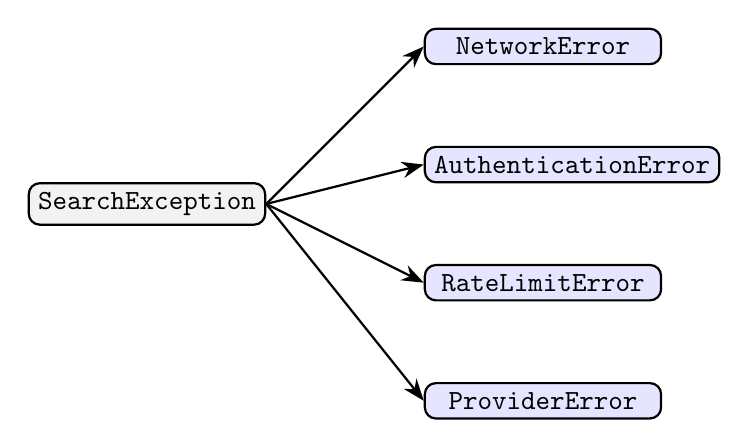
\begin{tikzpicture}[
      node distance=0.8cm and 2cm,
      base/.style={rectangle, draw, thick, rounded corners, minimum width=2.5cm, align=center, fill=black!5},
      child/.style={rectangle, draw, thick, rounded corners, minimum width=3cm, align=center, fill=blue!10},
      arrow/.style={-{Stealth[scale=1.2]}, thick}
    ]
    
    \node[base] (base_ex) {\texttt{SearchException}};
    
    \node[child, right=of base_ex, yshift=2cm] (net) {\texttt{NetworkError}};
    \node[child, right=of base_ex, yshift=0.5cm] (auth) {\texttt{AuthenticationError}};
    \node[child, right=of base_ex, yshift=-1cm] (rate) {\texttt{RateLimitError}};
    \node[child, right=of base_ex, yshift=-2.5cm] (prov) {\texttt{ProviderError}};
    
    \draw[arrow] (base_ex.east) -- (net.west);
    \draw[arrow] (base_ex.east) -- (auth.west);
    \draw[arrow] (base_ex.east) -- (rate.west);
    \draw[arrow] (base_ex.east) -- (prov.west);
  \end{tikzpicture}
  }
  \end{center}
\end{frame}

\begin{frame}{Why Custom Exceptions?}
  \begin{block}{Catching with Precision}
    A generic \texttt{requests.exceptions.ConnectionError} is an implementation detail. We wrap it in a \texttt{NetworkError}.
  \end{block}
  
  \begin{itemize}
      \item Our core engine should never import \texttt{requests} or \texttt{httpx} specific errors.
      \item This allows us to swap HTTP clients later without breaking the retry logic.
  \end{itemize}
\end{frame}

\begin{frame}{Implementation: `RateLimitError`}
  \begin{block}{The Payload}
    Some exceptions need to carry data, not just string messages.
  \end{block}
  
  \begin{itemize}
      \item Our \texttt{RateLimitError} stores the \texttt{retry\_after} integer (in seconds).
      \item This allows the outer orchestration loop to dynamically sleep for the exact required duration.
  \end{itemize}
\end{frame}

\begin{frame}{Verification}
  \begin{alertblock}{Success Criteria}
    \begin{itemize}
        \item Raising a \texttt{RateLimitError} successfully inherits from \texttt{SearchException}.
        \item The \texttt{retry\_after} attribute is accessible by the caller.
    \end{itemize}
  \end{alertblock}
\end{frame}

\end{document}
